\documentclass[a4paper,10pt]{book}
\usepackage[utf8x]{inputenc}
\usepackage{graphicx}
\DeclareGraphicsRule{.eps}{eps}{}{}
\usepackage{hyperref}

\title{Trasduttori}
\author{Federico Vaga}
\date{Giugno 2012}

\begin{document}
% stampa la licenza CC BY-NC-SA_2.5_IT
\input{licenza/CreativeCommons/BY-NC-SA_2.5_IT/BY-NC-SA_2.5_IT.tex}

\tableofcontents
\listoffigures

\part{Trasduttori}
\chapter{Introduzione}
Lo scopo di un trasduttore è quello di trasformare un segnale di
natura fisica in un segnale elettrico; per fare questo i trasduttori
si basano su principi fisici.
Per descrivere le caratteristiche di un trasduttore possiamo
catalogarle in statiche (cioè proprie del trasduttore) e dinamiche
(cioè che dipendono dal processo al quale lo si applica).
Fra le caratteristiche statiche abbiamo:
\begin{itemize}
 \item \textit{Sensibilità}: rapporto fra la variazione di grandezza
elettrica e di grandezza fisica.
	\[ \frac{\Delta GE}{\Delta GF} \]
 \item \textit{Risoluzione}: cioè la minima variazione valutabile
della grandezza fisica. Di conseguenza avremo una rappresentazione
della grandezza fisica con un segnale a gradini. Questa è la diretta
conseguenza del passaggio dallo spazio continuo (analogico/fisico)
allo spazio discreto (digitale).
 \item \textit{Soglia}: il minimo valore della grandezza fisica
misurabile.
 \item \textit{Range}: intervallo di valori della grandezza fisica in
esame che il trasduttore può misurare.
 \item \textit{Isteresi}: massima differenza tra due cammini di
andata e di ritorno dell'uscita del trasduttore durante un ciclo che
raggiunge gli estremi del range.
 \item \textit{condizioni ambientali}: condizioni ambientali che
garantiscono il corretto funzionamento; se il trasduttore viene fatto
lavorare fuori dalle condizioni nominali si possono generare errori.
 \item \textit{errore}: differenza fra il comportamento reale e
quello ideale, a questo viene anche associata una
 \item \textit{banda d'errore}: è una regione in cui i valori reali
possono differire da quelli ideali.
\end{itemize}

Le caratteristiche dinamiche di un trasduttore dipendono dal
funzionamento del processo al quale viene applicato, il problema
principale è verificare se il trasduttore scelto è in grado di seguire
fedelmente le variazioni del processo; per capirlo vengono forniti i
diagrammi di Bode della sensibilità del trasduttore (fig. d) e nel
caso in cui il trasduttore non riesca ad operare a frequenze troppo
basse viene fornita la banda di applicabilità (fig. e). Altra
caratteristica dinamica importante è l'affidabilità del trasduttore,
cioè la capacità di sopportare sovraccarichi, la vita media del
trasduttore.
\chapter{Trasduttori di posizione lineare}
\section{Potenziometro a filo avvolto}\label{sec:filoavvolto}
Si tratta di un filo di lega metallica con resistività e dimensioni
stabili che viene avvolto lungo un cilindro rigido; un cursore,
anch'esso metallico, viene poso sopra al cilindro di modo che possa
fare contatto sul filo avvolto e sarà proprio su questo cursore che
verrà prelevata la tensione di riferimento per il campionamento. In
figura \ref{fig:filoavvolto} è possibile vederne una
rappresentazione schematica, mentre in figura \ref{fig:potenziometro}
la rappresentazione circuitale.

\begin{figure}[htbp]
	\centering
	\includegraphics[scale=0.5]
			{img/filoavvolto.png}
	\caption{Potenziometro a filo avvolto\label{fig:filoavvolto}}
\end{figure}

\begin{figure}[htbp]
	\centering
	\includegraphics[scale=0.5]
			{img/potenziometro.pdf}
	\caption{Potenziometro\label{fig:potenziometro}}
\end{figure}

Per ricavare il valore della tensione in uscita V basta applicare la
regola del partitore di tensione, immaginando che le due resistenze
siano rappresentate: una dalla parte alla sinistra del cursore (sulla
quale si preleva la misura della tensione) e l'altra dalla parte alla
destra del cursore come in figura \ref{fig:potenziometroequiv}.

\begin{figure}[htbp]
	\centering
	\includegraphics[scale=0.5]
			{img/potenziometro-equiv.pdf}
	\caption{Circuito equivalente
per il potenziometro\label{fig:potenziometroequiv}}
\end{figure}

Il problema è ora quantificare il valore di queste
due resistenze e metterlo in relazione con con lo spostamento $X$ del
cursore rispetto all'inizio (cioè quando il cursore è tutto a
sinistra). Ora indichiamo con $L$ la lunghezza del potenziometro e
calcoliamo $V$:

\[ R = \frac{L}{S}\rho \rightarrow R_1=\frac{L-S}{S}\rho,
R_2=\frac{S}{S}\rho \]
\[V=E\frac{R_2}{R_1+R_2}=E\frac{\rho\frac{X}{S}}{\rho\frac{L-X}{S}
+ \rho\frac{X}{S}}= E \frac{X}{L}\]

Da qui la relazione che lega $V$ con $X$:

	\[\frac{X}{L} = \frac{V}{E}\]

\subsection{Vantaggi}
Il primo vantaggio è la linearità: la resistività uniforme del cavo
permette una distribuzione di potenziale che è lineare nello spazio.
Un secondo vantaggio, è la possibilità di ottenere un segnale
elettrico di ampiezza desiderato. Il trasduttore è insensibile alla
variazione di temperatura se questa avviene uniformemente su l'intero
trasduttore.
\subsection{Svantaggi}
La risoluzione limitata dovuto allo spazio vuoto fra due avvolgimenti
del filo metallico, inoltre in questo spazio si può perdere la misura.
La vita media breve a causa dell'usura generata dal movimento del
cursore e, infine, la forza necessaria per vincere l'attrito generato
dal movimento del contatto provoca un'alterazione del sistema sotto
misura, quindi possono esserci possibili isteresi.

\section{Potenziometro a strato di carbonio}\label{sec:potcarbonio}
Il funzionamento è del tutto analogo a quello del potenziometro a filo
avvolto\ref{sec:filoavvolto} con la differenza che a fornire la
resistenza c'è ora uno strato di carbonio sul quale va a posizionarsi
il cursore.

\begin{figure}[htbp]
	\centering
	\includegraphics[scale=0.5]
			{img/potenziometro-carbonio.pdf}
	\caption{Potenziometro a
strato di carbonio\label{fig:potenziometro-carbonio}}
\end{figure}

Il vantaggio introdotto è che ora la risoluzione non è più
a scalino ma è lineare lontano dagli estremi, lo svantaggio invece è
la vita molto breve dovuto al consumo dello strato di carbonio causato
dallo sfregamento del cursore su di esso.

\section{Potenziometro elettro-ottico
(fotopotenziometro)}\label{sec:elettrottico}
Essendo un potenziometro, il suo comportamento è analogo a quello
visto per il potenziometro a filo avvolto\ref{sec:filoavvolto}, cambia
solo il modo in cui viene realizzato. La realizzazione di un
potenziometro elettro-ottico prevede di unire un film resistivo con
una striscia di materiale foto-conduttore e del materiale conduttore.

\begin{figure}[htbp]
	\centering
	\includegraphics[scale=0.5]
			{img/fotopotenziometro.png}
	\caption{Foto-potenziometro\label{fig:fotopotenziometro}}
\end{figure}

A questo punto sopra a questi tre elementi viene posta una lamina
tagliata. Attraverso la lamina viene fatta passare la luce che farà
passare la corrente nel punto in cui il materiale fotoconduttore è
illuminato permettendo così di prelevare la tensione V sul materiale
conduttore.

\subsection{Vantaggi}
Il principale vantaggio è l'assenza di contati meccanici striscianti
e di conseguenza una vita più lunga del trasduttore. Questo tipo di
potenziometro offre una maggiore risoluzione.
\subsection{Svantaggi}
Questo tipo di potenziometro garantisce una linearità inferiore,
inoltre è molto più complesso, quindi costoso, da realizzare.
Richiede il buio totale in quanto le infiltrazioni di luce esterna
potrebbero introdurre errori.

\section{Trasduttore capacitivo}\label{sec:potcapacitivo}
Esso è costituito da tre armature di metallo di cui due fisse ed
allineate e una mobile che si muove sopra le altre due creando così
due capacità differenti che variano a seconda dell'area dell'armatura
mobile che copre una delle due armature. In figura
\ref{fig:potcapacitivo} una rappresentazione schematica.

\begin{figure}[htbp]
	\centering
	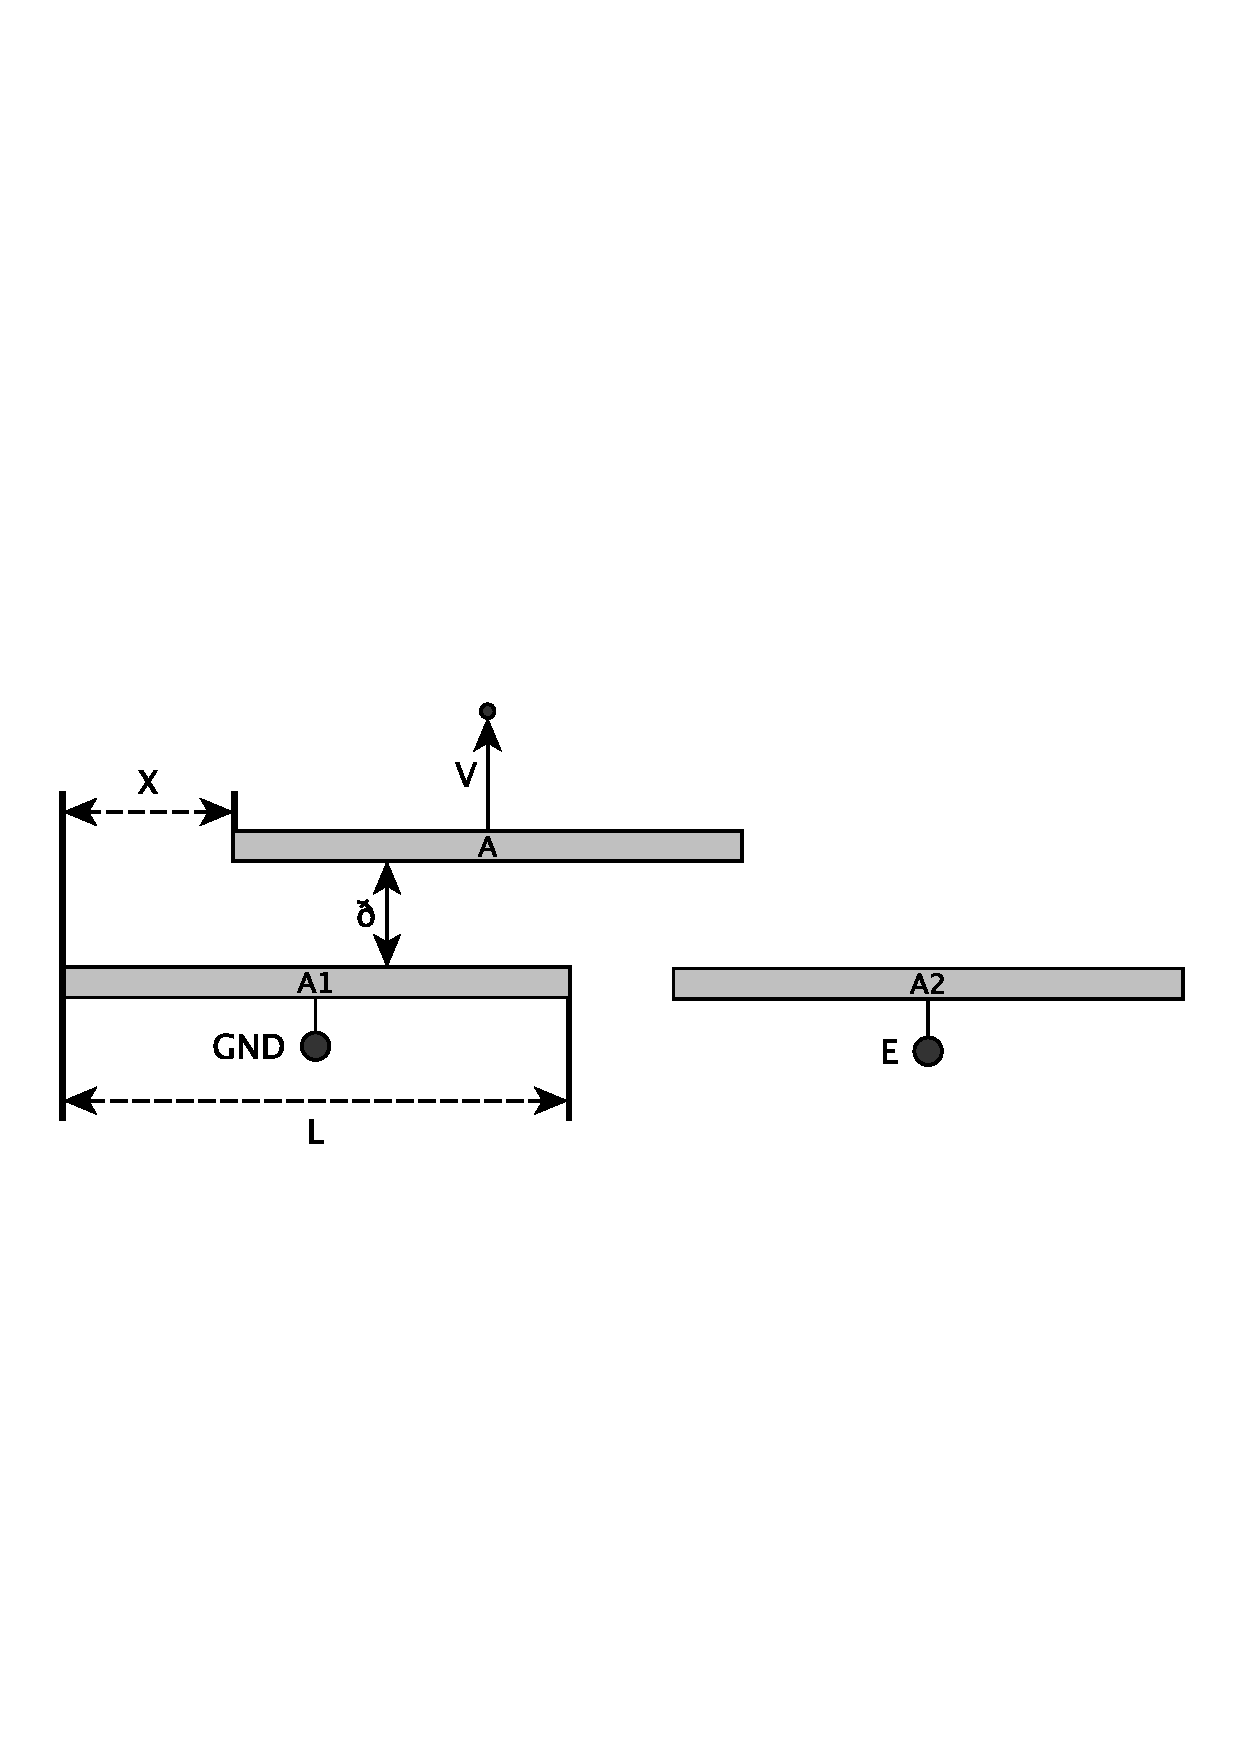
\includegraphics[scale=0.5]{img/potenziometro-capacitivo.pdf}
	\caption{Potenziometro capacitivo\label{fig:potcapacitivo}}
\end{figure}

In questo modo sempre col partitore di tensione possiamo misurare lo
spostamento. In figura \ref{fig:potcapacitivoequiv} il circuito
equivalente.

\begin{figure}[htbp]
	\centering
	\includegraphics[scale=0.5]
			{img/potenziometro-capacitivo-equiv.pdf}
	\caption{Circuito equivalente
del trasduttore capacitivo\label{fig:potcapacitivoequiv}}
\end{figure}

Le capacità $C_1$ e $C_2$ sono le capacità che si vengono a creare
dalla sovrapposizione delle armature $A_1$ e $A_2$ con l'armatura $A$.
$H$ indica la profondità dell'armatura.

	\[
	C_1=\frac{H (L-x)}{\delta}\varepsilon_0,
	C_2 =\frac{Hx}{\delta}\varepsilon_0
	\]
	\[
	V=E\frac{\frac{1}{sC_1}}{\frac{1}{sC_1}+\frac{1}{sC_2}}
	 =E\frac{C_2}{C_1+C_2}
	 =E\frac{\frac{Hx}{\delta}\varepsilon_0}
		{\frac{Hx}{\delta}\varepsilon_0+
				\frac{H(L-x)}{\delta}\varepsilon_0}
	 =E\frac{x}{L}
	\]

\subsection{Vantaggi}
I vantaggi sono gli stessi del potenziometro
elettro-ottico\ref{sec:elettrottico}
\subsection{Svantaggi}
Questo trasduttore soffre di scarsa linearità agli estremi; inoltre
si hanno problemi di carico inquanto l'impedenza del condensatore è
elevata, questo suggerisce l'utilizzo di un buffer ad alta
impedenza d'ingresso. Per ultimo, quando si lavora in
tensione alternata si rende necessario un circuito raddrizzatore a
valle del potenziometro.

\subsection{Variazione di impedenza}
Un alternativa è quella di usare un trasduttore di posizione
capacitivo a variazione d'impedenza, costruito come due cilindri che
si inseriscono uno dentro l'altro e muovendoli varia la capacità come
$C=KX$ e quindi anche l'impedenza.

\begin{figure}[htbp]
	\centering
	\includegraphics[scale=0.5]
			{img/potenziometro-capacitivo-2.png}
	\caption{Potenziometro
capacitivo alternativo\label{fig:potcapacitivoalt}}
\end{figure}

\section{Trasformatore differenziale}
La trasduzione si basa sul principio della mutua induttanza variabile:
per realizzare ciò si utilizza un avvolgimento primario e due
avvolgimenti secondari di accoppiamento. L'accoppiamento avviene
tramite un cilindro ferromagnetico di sezione $S$ e lunghezza $L$ che
si muove fra il primario e il secondario.

\begin{figure}[htbp]
	\centering
	\includegraphics[scale=0.5]
			{img/trasformatore-differenziale.png}
	\caption{Trasformatore differenziale\label{fig:trasdiff}}
\end{figure}

Le due induttanze secondarie sono in serie ma in opposizione di fase,
ne risulta quindi che $V_{out}=E_1-E_2$. La direzione dello
spostamento si deduce a seconda che $V_out$ sia in fase con $e$ o
meno. Indichiamo con $N_1$ il numero di spire coperte dal cilindro sul
primo solenoide e $N_2$ il numero di spire coperte dal cilindro sul
secondo, mentre con $B$ il campo magnetico del cilindro
ferromagnetico. Definiamo quindi il flusso di $B$ attraverso ad una
singola spira (anche lei di sezione $S$) e quindi il flusso sui
solenoidi 1 e 2:

	\[\phi=BS\]
	\[\phi_1=\phi N_1, \phi_2=\phi N_2 \]

A questo punto possiamo definire la forza elettro motrice sui due
solenoidi:

	\[E_1=j\omega\phi_1, E_2=j\omega\phi_2 \]

La tensione in uscita sarà quindi data da:

	\[V_out = E_1 - E_2 = j\omega\phi[N_1 - N_2]\]

Prendendo come posizione di riferimento dello spostamento, il punto
centrale fra i due secondari, avremo che in condizione di riposo il
cilindro compre metà spire del primo solenoide e metà del secondo,
quindi:

	\[N_1 = [\frac{L}{2}+X]n, N_1 = [\frac{L}{2}-X]n\]

dove $n$ è la densità di spire dei solenoidi. Da questa
considerazione ne consegue che:

	\[V_out=j\omega\phi 2nX\]

L'uso di questo trasduttore è consigliato a base frequenze perché vi
è un'impedenza in uscita minore ($j\omega Z_L$).
Da notare che avviene un'inversione di fase per spostamenti negativi;
in figura \ref{fig:trasdifffase} la rappresentazione del segnale in
uscita.

\begin{figure}[htbp]
	\centering
	\includegraphics[scale=0.5]
			{img/trasformatore-differenziale-fase.png}
	\caption{Segnale in uscita da un trasformatore
differenziale\label{fig:trasdifffase}}
\end{figure}

\section{Trasduttore ad induttanza variabile}
Vengono posti in vicinanza due pezzi di materiale ferromagnetico, uno
a ferro di cavallo e l'altro a forma di barretta; quest'ultima è
mobile, quindi è possibile avvicinarla o allontanarla misurando così
lo spostamento.

\begin{figure}[htbp]
	\centering
	\includegraphics[scale=0.5]
			{img/induttanza-variabile.png}
	\caption{Trasduttore ad induttanza
variabile\label{fig:trasdifffase}}
\end{figure}

Possiamo ora calcolare la riluttanza del circuito ferromagnetico;
teniamo conto però solo dei tratti $L_5$ ed $L_3$ in quanto gli unici
significativi per la determinazione della distanza ($S$ indica la
sezione del ramo e $\mu$ la permeabilità, $\mu_0$ la permeabilità
del vuoto).

	\[\Re=\sum_i{\frac{L_i}{S_im_i}}\]
	\[\Re=\frac{L_2}{S_2\mu_3} + \frac{L_5}{S_5\mu_5}
	     =2\frac{X}{S\mu_0}\]

La riluttanza può essere misurata avvolgendo un certo numero di spire
attorno al ramo $L_1$; le spire vengono disposte con una densità $n$.
Ne risulta che l'induttanza corrisponde a:

	\[
	L=\frac{n\phi}{I}
	 =\frac{\frac{n^2i}{\Re}}{i}
	 =\frac{n^2}{\Re}
	 =\frac{n^2S\mu_0}{2X}
	\]
Da qui possiamo ricavare l'ammettenza:

	\[Y=Z^{-1}=\frac{1}{\omega L}=\frac{2X}{\omega n^2S\mu_0}\]

Ne consegue che alimentando il circuito e misurando la
corrente $I=VY$, questa varierà al variare della distanza $X$

\subsection{Vantaggi}
La possibilità di regolare l'impedenza variando il numero di
spire avvolte sul materiale ferromagnetico (su $L_1$ per la
precisione) e la possibilità di fare misure di induttanza a frequenze
relativamente basse.
\subsection{Svantaggi}
La linearità peggiora più ci si allontana dal nucleo e
problemi di misura in alternata. Inoltre in corrente alternata abbiamo
problemi di misura.

\subsection{Trasduttore ad induttanza variabile alternativo}
Per colmare il difetto della linearità è possibile porre la barra
ferromagnetica fra due ferri di cavallo di modo che se peggiora
allontanandosi da uno, migliora avvicinandosi all'altro.

\begin{figure}[htbp]
	\centering
	\includegraphics[scale=0.5]
			{img/induttanza-variabile-2.png}
	\caption{Trasduttore ad induttanza
variabile alternativo\label{fig:trasdifffase}}
\end{figure}
\chapter{Trasduttori di posizione angolare}
\section{Potenziometro circolare}
Il funzionamento è identico a quello di posizione lineare cambia il
fatto che ora si misura un angolo e non una distanza quindi la
relazione ora è la seguente:

	\[V=E\frac{\theta}{360\textdegree}\]

\subsection{Vantaggi}
L'unico vantaggio è la linearità fra la tensione fornita e l'angolo
misurato.
\subsection{Svantaggi}
Gli svantaggi sono, invece, l'ambiguità fra l'inizio e la fine (il
cursore passa da 360 a 0 gradi) e l'esistenza di una zona morta nella
quale non si può misurare per via dell'assenza di contatti.

% \section{Synchro} % FIXME tosto
\section{Encoder binario ed a codice di Gray}
Tramite un encoder è possibile misurare numericamente l'angolo
rilevato, per farlo si utilizza un disco così costituito: tanti
settori quanti sono gli angoli misurabili e tante corone quanti sono i
bit necessari per determinare tutti gli angoli misurabili. Dopo la
divisione alcune aree vengono oscurate per identificare gli zero della
codifica binario o gray. Il codice gray viene utilizzato quando si
vuole eliminare l'ambiguità fra una codifica e l'altra.

\begin{figure}[htbp]
	\centering
	\includegraphics[scale=0.5]
			{img/encoder.png}
	\caption{Encoder binari ed a codice di
Gray\label{fig:encored}}
\end{figure}

Per la rilevazione della codifica vengono usate tante coppie di LED e
foto-transistor quante sono le corone utilizzate; dopo di che, vengono
opportunamente allineati di modo che ogni coppia faccia riferimento
solo ad una corona. Al movimento della corona grazie alle parti scure
è possibile rilevare la codifica dell'angolo.

\section{Encoder incrementale}
Questo tipo di encoder si differenzia dal precedente per l'utilizzo
di solo due corone concentriche suddivise in settori sfasati di un
quarto di periodo.

\begin{figure}[htbp]
	\centering
	\includegraphics[scale=0.5]
			{img/encoderincr.png}
	\caption{Encoder incrementale\label{fig:encored}}
\end{figure}

In questo modo è possibile riconoscere gli incrementi e i decrementi
di angolo e quindi calcolare l'angolo finale. Indichiamo con $P$ il
fronte positivo e con $N$ il fronte negativo del segnale e con $S_1$
la corona esterna e con $S_2$ la corona interna; ne risulta la
seguente tabella di incrementi:

\begin{center}
\begin{tabular}{lll}
$S_1$ & $S_2$ & incremento\\
P & 0 & +1\\
P & 1 & -1\\
N & 0 & -1\\
N & 1 & +1\\
0 & P & -1\\
1 & P & +1\\
0 & N & +1\\
1 & N & -1
\end{tabular}
\end{center}

A partire dalla posizione di riposo, sarà facile calcolare l'angolo
ottenuto nelle rotazioni.

\chapter{Trasduttori di velocità}
\section{Trasduttore elettromagnetico}
Esso è realizzato da un solenoide entro il quale viene inserito un
magnete permanente. Il magnete effettua un movimento all'interno del
solenoide; da questo movimento sappiamo ricavare la velocità
calcolando la derivata dello spostamento effettuato nel tempo.

%figura

Come per il trasformatore differenziale \ref{sec:trasdiff},
calcoliamo il flusso del campo magnetico all'interno delle spire
coperte dal magnete. La variazione del flusso ci indica lo
spostamento del magnete, e quindi derivando questa quantità rispetto
al tempo, otteniamo la velocità:

	\[V=-\frac{d(N_c\phi_B)}{dt}= -n\phi_B\frac{dx}{dt}
	   =-n\phi_B v\]


\section{Dinamo tachimetrica}
Il rotore è fisicamente costituito da un materiale ad elevatissima
permeabilità magnetica su cui è avvolto ad elica un filo chiuso su sé
stesso e connesso in punti situati ad intervalli regolari.
Sui segmenti del collettore sono poste delle spazzole su cui striscia
il rotore, queste poi sono collegate ai morsetti della macchina.

\begin{figure}[htbp]
	\centering
	\includegraphics[scale=0.5]
			{img/dinamo.png}
	\caption{Struttura di una dinamo tachimetrica
\label{fig:dianmo}}
\end{figure}

Il rotore ruota in un campo magnetico generato da un magnete
permanente. Essendo il rotore ad alta permeabilità magnetica, tutte le
linee di forza del campo magnetico B, che partono dai poli del
magnete, si concentrano entro il rotore. Posizionando le spazzole
nella parte alta e nella parte bassa riusciamo a ricavare una forza
elettro motrice non nulla che ci può indicare la velocità di
rotazione. Consideriamo la tensione fornita da una singola spira:

	\[e = \overrightarrow{v} \wedge \overrightarrow{B} \times
\overrightarrow{L} \]

dove $\overrightarrow{v}$ è la velocità tangenziale del rotore,
$\overrightarrow{B}$ il campo magnetico e $\overrightarrow{L}$ lo
spessore del rotore. Ne consegue che il contributo di una singola
spira soggetta al campo magnetico $B$ è:

	\[e=vBL\]

Data la simmetria del rotore la somma delle f.e.m. indotte è nulla;
l'uso delle spazzole però consente di ottenere una f.e.m. non nulla
in quanto divide in due rami il rotore. La situazione è
modellabile come due serie di generatori di tensione messi in
parallelo. Ne risulta che la f.e.m. indotta totale è:

	\[E=e_{medio}\frac{N}{2}= vB_{medio}L\frac{N}{2}\]

dove $N$ è il numero totale di spire. Ricaviamo ora il valore della
f.e.m. in funzione del numero di giri del rotore:

	\[\phi_B=\int BdS=B_{medio}S=L\pi r B_m \]
	\[E=v\frac{\phi_B}{L \pi r}L\frac{N}{2}\]

Sappiamo che $v=\omega r= 2\pi n r$ dove $n$ è il numero di giri al
secondo, quindi possiamo scrivere:

	\[E=\phi_B n N\]

La f.e.m. indotta nella bobina è sempre sinusoidale se il campo B è
uniforme, ma ogni volta che il flusso concatenato è massimo (e quindi
la f.e.m. indotta ha il valore zero) il contatto s'inverte, in modo
che ogni spazzola è sempre in contatto con un semi-anello che ha la
stessa polarità. Con questo la tensione fra le spazzole, e quindi fra
i morsetti A e B della macchina, ha sempre il medesimo segno.
Aumentando il numero di spire, la tensione che ne risulta è pressapoco
continua, questo però non impedisce l'ondulazione (cioè il passaggio
fra un elettrodo e un altro). Con la dinamo tachimetrica purtroppo non
è possibile utilizzare dei filtri per eliminare il rumore dato che
questo dipende dalla velocità con cui si muove il rotore.

\section{Alternatori tachimetrici}
Un trasduttore di questo tipo è costituito da un magnete rotante che
genera tensioni alternata su degli avvolgimenti fissi.

\begin{figure}[htbp]
	\centering
	\includegraphics[scale=0.5]
			{img/alternatoretachi.png}
	\caption{Alternatore tachimetrico\label{fig:altachi}}
\end{figure}


La frequenza e l'ampiezza della tensione alternata rilevata sono
proporzionali alla velocità di rotazione. La misura della velocità è
ricavabile da entrambe le variabili.

%FIXME conti

\section{Generatori ad induzione}

%FIXME da fare

\section{Trasduttore a carica e scarica capacitiva}
Si tratta di un collettore rotante a quattro segmenti con quattro
elettrodi fissi. Due dei segmenti sono collegati assieme per mezzo di
un condensatore. Due elettrodi sono alimentati e i rimanenti due sono
collegati ad un carico.

\begin{figure}[htbp]
	\centering
	\includegraphics[scale=0.5]
			{img/caricascaricacapacitiva.png}
	\caption{Trasduttore a carica e scarica capacitiva
\label{fig:carscarcap}}
\end{figure}

Durante la rotazione il condensatore si carica quando i due segmenti
toccano gli elettrodi alimentati, mentre si scarica quando tocca gli
elettrodi con il carico. La velocità di rotazione viene determinata
attraverso la frequenza degli impulsi di carico del condensatore
rilevati sul ramo a cui è collegato il carico ($U$). Questa misura è
ottenibile mediante l'uso di un frequenzimetro. In alternativa al
frequenzimetro è possibile utilizzare l'integratore approssimato
mostrato in figura \ref{fig:carscarint}:

\begin{figure}[htbp]
	\centering
	\includegraphics[scale=0.5]
			{img/caricascaricaintegra.png}
	\caption{Integratore approssimato per la rilevazione della
frequenza
\label{fig:carscarint}}
\end{figure}

Ponendo $R'C' >> \frac{T}{2}$ otterremo che il valore della tensione
in uscita $V_o$ corrisponderà al valore medio della tensione in
uscita sul trasduttore:

	\[ V_o = 2ERC\frac{1}{T} = 2fERC \]

Ovviamente la velocità di rotazione ha un limite superiore dovuto al
tempo di carico/scarico del condensatore. Inoltre nel caso
dell'integratore approssimato, la precisione diminuisce vicino a
questo limite. Un frequenzimetro garantisce una migliore precisione.

\section{Trasduttore elettro-ottico}
Con l'ausilio di un traduttore encoder e un'opportuna logica è
possibile calcolare la angolare oltre che il senso di rotazione.
\chapter{Trasduttori di accelerazione}
\section{Accelerometro massa-molla}
Consiste in una scatola in cui è presente una piccola massa che può
muoversi orizzontalmente e che è soggetta ad un'azione di richiamo da
parte di una molla; nello stesso contenitore è presente un trasduttore
di posizione lineare che misura la posizione della massa. Indicando
con $x$ lo spostamento relativo della massa $m$ e applicando le leggi
della fisica per le molle ($k$ costante elastica della molla) possiamo
facilmente ricavare l'accelerazione $a$:

	\[F=ma=-kx \Rightarrow x=-\frac{ma}{k}\]

Data che c'è proporzionalità fra lo spostamento $x$ e l'accelerazione
$a$, possiamo definire la sensibilità del trasduttore come rapporto
fra lo spostamento e l'accelerazione:

	\[x=-\frac{ma}{k} \Rightarrow \frac{x}{a}=-\frac{m}{k}\]

\section{Servo-accelerometro}
Un servo-accelerometro è costituito da una massa $m$ collegata ad un
motore in continua $C$ di modo da far oscillare il rotore del motore.
Quando la massa subisce un'accelerazione questa si sposta e genera
una coppia proporzionale all'accelerazione. Un trasduttore di
posizione lineare rileva lo spostamento della massa rispetto alla sua
posizione di riposo; il segnale in uscita da questo trasduttore è
applicato ad un amplificatore la cui corrente in uscita è applicata
al motore che genera una coppia uguale e contraria a quella fornita
dalla massa. In questo modo la massa ritorna alla sua posizione di
riposto. La tensione misurata sul carico situalo fra il motore e
l'amplificatore ci darà una tensione proporzionale all'accelerazione.

\section{Accelerometro piezoelettrico}
Il principio alla base di un accelerometro piezoelettrico è lo stesso
del massa-molla con l'aggiunta di un cilindretto di materiale
piezoelettrico che assolve le funzioni di richiamo della molla e di
misurazione dello spostamento.
%FIXME trattazione fisica del piezo

\section{Accelerometro MEMS}
Gli accelerometri di questo tipo sono realizzati con tecnologia MEMS
(Micro-Electro-Mechanical-System). Questo tipo di tecnologia permette
di realizzare sensori, attuatori e altri dispositivi elettrinici
mediante un processo di lavorazione di uno strato di silicio.
Un accelerometro di tipo MEMS ha lo stesso principio del massa-molla
ma è realizzato mediante l'uso di gas. All'interno dell'accelerometro
viene creata un piccola bolla di gas riscaldato che si muove in
funzione degli spostamenti. Mediante dei sistemi di misurazione della
temperatura, distribuiti dentro all'accelerometro, è possibile
individuare lo spostamento della bolla quindi ricavare l'accelerazione
che ne ha generato lo spostamento.

\part{Attuatori}
\chapter{Introduzione}
Lo scopo di un trasduttore è quello di trasformare un segnale di
natura fisica in un segnale elettrico; per fare questo i trasduttori
si basano su principi fisici.
Per descrivere le caratteristiche di un trasduttore possiamo
catalogarle in statiche (cioè proprie del trasduttore) e dinamiche
(cioè che dipendono dal processo al quale lo si applica).
Fra le caratteristiche statiche abbiamo:
\begin{itemize}
 \item \textit{Sensibilità}: rapporto fra la variazione di grandezza
elettrica e di grandezza fisica.
	\[ \frac{\Delta GE}{\Delta GF} \]
 \item \textit{Risoluzione}: cioè la minima variazione valutabile
della grandezza fisica. Di conseguenza avremo una rappresentazione
della grandezza fisica con un segnale a gradini. Questa è la diretta
conseguenza del passaggio dallo spazio continuo (analogico/fisico)
allo spazio discreto (digitale).
 \item \textit{Soglia}: il minimo valore della grandezza fisica
misurabile.
 \item \textit{Range}: intervallo di valori della grandezza fisica in
esame che il trasduttore può misurare.
 \item \textit{Isteresi}: massima differenza tra due cammini di
andata e di ritorno dell'uscita del trasduttore durante un ciclo che
raggiunge gli estremi del range.
 \item \textit{condizioni ambientali}: condizioni ambientali che
garantiscono il corretto funzionamento; se il trasduttore viene fatto
lavorare fuori dalle condizioni nominali si possono generare errori.
 \item \textit{errore}: differenza fra il comportamento reale e
quello ideale, a questo viene anche associata una
 \item \textit{banda d'errore}: è una regione in cui i valori reali
possono differire da quelli ideali.
\end{itemize}

Le caratteristiche dinamiche di un trasduttore dipendono dal
funzionamento del processo al quale viene applicato, il problema
principale è verificare se il trasduttore scelto è in grado di seguire
fedelmente le variazioni del processo; per capirlo vengono forniti i
diagrammi di Bode della sensibilità del trasduttore (fig. d) e nel
caso in cui il trasduttore non riesca ad operare a frequenze troppo
basse viene fornita la banda di applicabilità (fig. e). Altra
caratteristica dinamica importante è l'affidabilità del trasduttore,
cioè la capacità di sopportare sovraccarichi, la vita media del
trasduttore.


\end{document}
